
\section{觀念與公式}

\subsection{數列的基本概念}
數列是有序的數字序列,如$1, 4, 7, 10, \ldots$。\\
\textbf{表示法}:
\begin{itemize}
    \item 通項:$a_n$,如$a_n = 3n - 2$。
    \item 遞推:$a_n = a_{n-1} + d$,需給初值。
\end{itemize}
\textbf{類型}:等差、等比、費氏數列。\\
\textbf{應用}:描述規律變化。\\
\textbf{大學技巧}:用生成函數分析遞推數列。

\subsection{等差數列}
每項與前項差為常數$d$(公差)。\\
\textbf{公式}:
\begin{itemize}
    \item 通項:$a_n = a_1 + (n-1)d$。
    \item 總和:$S_n = \frac{n}{2} (a_1 + a_n)$ 或 $S_n = \frac{n}{2} [2a_1 + (n-1)d]$。
\end{itemize}
\textbf{性質}:線性增長。\\
\textbf{應用}:均勻增加問題。\\
\textbf{大學技巧}:用數學歸納法證總和公式。

\subsection{等比數列}
每項與前項比為常數$r$(公比)。\\
\textbf{公式}:
\begin{itemize}
    \item 通項:$a_n = a_1 r^{n-1}$。
    \item 總和:$S_n = a_1 \frac{1 - r^n}{1 - r}$($r \neq 1$)。
    \item 無限級數:若$|r| < 1$,$S_\infty = \frac{a_1}{1 - r}$。
\end{itemize}
\textbf{性質}:指數增長或衰減。\\
\textbf{應用}:利息、折舊。\\
\textbf{大學技巧}:判斷級數收斂性。

\subsection{級數}
數列項的和$S_n = a_1 + a_2 + \cdots + a_n$。\\
\textbf{類型}:
\begin{itemize}
    \item 有限級數:固定項數。
    \item 無限級數:需判斷收斂。
\end{itemize}
\textbf{應用}:累積總量。\\
\textbf{大學技巧}:泰勒級數近似函數。

\subsection{數學歸納法}
證明數列性質:
\begin{enumerate}
    \item 基礎步:驗證$n = 1$。
    \item 歸納步:假設$n = k$成立,證$n = k+1$。
\end{enumerate}
\textbf{應用}:證總和公式。\\
\textbf{大學技巧}:證複雜遞推關係。

\section{例題解析}

\subsection{例題1:等差數列(計算題)}
一等差數列首項$3$,公差$2$,求第10項與前10項和。\\
\textbf{解}:通項$a_n = 3 + (n-1) \cdot 2$,$a_{10} = 3 + 9 \cdot 2 = 21$。\\
總和$S_{10} = \frac{10}{2} (3 + 21) = 5 \cdot 24 = 120$。\\
\textbf{大學技巧}:驗證$a_{10} - a_9 = 2$。

\subsection{例題2:等比數列(應用題)}
一物品價值1000元,每年折舊20\%,求第5年價值與5年總價值。\\
\textbf{解}:$a_n = 1000 \cdot (0.8)^{n-1}$,$a_5 = 1000 \cdot (0.8)^4 = 409.6$元。\\
$S_5 = 1000 \frac{1 - (0.8)^5}{1 - 0.8} = 1000 \cdot \frac{1 - 0.32768}{0.2} = 3361.6$元。\\
\textbf{大學技巧}:無限折舊$S_\infty = \frac{1000}{0.2} = 5000$元。

\subsection{例題3:遞推數列(觀念題)}
費氏數列$a_1 = 1, a_2 = 1, a_n = a_{n-1} + a_{n-2}$,求$a_6$。\\
\textbf{解}:$a_3 = 2, a_4 = 3, a_5 = 5, a_6 = 8$。\\
\textbf{大學技巧}:黃金比例近似$a_n \approx \frac{\phi^n}{\sqrt{5}}$,$\phi = \frac{1 + \sqrt{5}}{2}$。

\subsection{例題4:數學歸納法}
證$S_n = \frac{n}{2} [2a_1 + (n-1)d]$。\\
\textbf{解}:$n = 1$,$S_1 = a_1$成立。假設$n = k$成立,$n = k+1$:
\[
S_{k+1} = S_k + a_{k+1} = \frac{k}{2} [2a_1 + (k-1)d] + [a_1 + kd] = \frac{k+1}{2} [2a_1 + kd]
\]
成立。\\
\textbf{大學技巧}:用連續和推導。

\section{圖形展示}
等比數列$a_n = 2 \cdot (0.5)^{n-1}$:
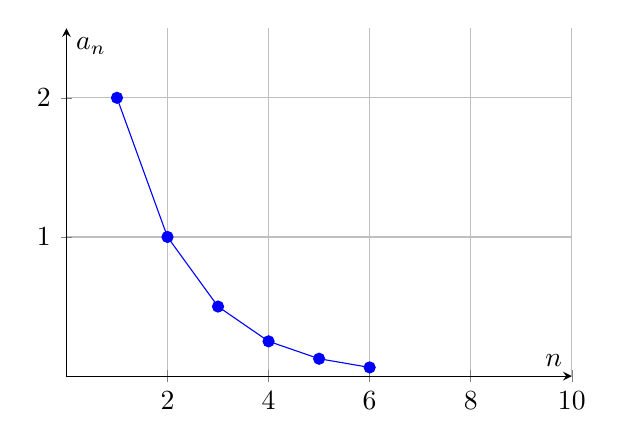
\begin{tikzpicture}
    \begin{axis}[
        axis lines=middle,
        xlabel=$n$,
        ylabel=$a_n$,
        xmin=0, xmax=10,
        ymin=0, ymax=2.5,
        grid=both,
        width=8cm, height=6cm
    ]
    \addplot[mark=*, blue] coordinates {(1,2) (2,1) (3,0.5) (4,0.25) (5,0.125) (6,0.0625)};
    \end{axis}
\end{tikzpicture}

\section{題庫}
\begin{enumerate}[label=\arabic*.]
    % 計算題 (10)
    \item 求等差數列$a_1 = 5, d = 3$的$a_{10}$。
    \item 求等比數列$a_1 = 2, r = 2$的$S_5$。
    \item 若$a_n = 4n - 1$,求$S_{10}$。
    \item 求等差數列$a_1 = 1, a_5 = 9$的$d$。
    \item 求等比數列$a_1 = 3, r = \frac{1}{2}$的$a_6$。
    \item 若$a_1 = 2, d = -1$,求$S_{20}$。
    \item 求$a_n = a_{n-1} + 3, a_1 = 1$的$a_8$。
    \item 求等比數列$a_1 = 1, r = -2$的$S_4$。
    \item 若$a_1 = 10, d = 2$,求$a_{15}$。
    \item 求等比數列$a_1 = 4, r = 0.5$的$S_\infty$。
    % 應用題 (10)
    \item 一存款首年1000元,每年增200元,求第10年總額。
    \item 一球從10公尺落下,每次反彈前高0.8倍,求總距離。
    \item 若$a_1 = 1, a_n = 2a_{n-1}$,求$S_6$。
    \item 一數列$a_1 = 3, d = 4$,求第幾項為$35$。
    \item 一物品首年值5000元,年折舊10\%,求5年總值。
    \item 若$S_n = 3n^2 + 1$,求$a_n$。
    \item 一等差數列$a_1 = 2, S_{10} = 110$,求$d$。
    \item 一等比數列$a_1 = 2, S_5 = 62$,求$r$。
    \item 若$a_1 = 1, a_n = a_{n-1} + n$,求$a_5$。
    \item 一數列$a_1 = 5, r = \frac{1}{3}$,求$S_\infty$。
    % 觀念題 (10)
    \item 證等差數列$S_n = \frac{n}{2} (a_1 + a_n)$。
    \item 等比數列$|r| > 1$時,$S_\infty$是否存在?
    \item 說明數學歸納法的步驟。
    \item 若$a_n = a_{n-1} + 2$,求通項。
    \item 證$S_n = a_1 \frac{1 - r^n}{1 - r}$。
    \item 等差數列總和公式有幾種形式?
    \item 若$a_n = 2^n$,求$S_n$。
    \item 說明費氏數列的遞推關係。
    \item 若$S_n = n(n+1)$,求$a_n$。
    \item 等比數列收斂條件為何?
    % 進階題 (10)
    \item 求$a_1 = 1, d = 3$,$S_n = 100$的$n$。
    \item 若$a_1 = 2, r = 3$,求$a_5$與$S_5$。
    \item 求$a_n = a_{n-1} + a_{n-2}, a_1 = 1, a_2 = 1$的$a_7$。
    \item 若$S_n = 2^n - 1$,求$a_n$。
    \item 求$a_1 = 4, d = -2$,$a_n = -10$的$n$。
    \item 若$a_1 = 1, r = \frac{1}{2}$,求$n$使$S_n > 1.9$。
    \item 求$a_1 = 3, d = 5$,$S_{10}$。
    \item 若$a_1 = 2, r = -1$,求$S_{100}$。
    \item 求$a_n = 3n^2 - 1$的$S_5$。
    \item 若$a_1 = 1, a_n = 3a_{n-1}$,求$a_6$。
    % 挑戰題 (20)
    \item 一等差數列$a_1 = 2, a_{10} = 20$,求$S_{10}$。
    \item 若$a_1 = 1, r = 2$,求$n$使$a_n > 1000$。
    \item 求$a_1 = 5, d = -3$,$S_n = -20$的$n$。
    \item 若$a_1 = 3, r = \frac{1}{2}$,求$n$使$S_n > 5.9$。
    \item 求$a_n = a_{n-1} + 2n, a_1 = 1$的$a_5$。
    \item 若$S_n = \frac{n(n+1)(2n+1)}{6}$,求$a_n$。
    \item 求$a_1 = 1, r = -2$,$S_6$。
    \item 若$a_1 = 4, d = 2$,求$n$使$S_n > 100$。
    \item 求$a_n = 2^n$的$S_{10}$。
    \item 若$a_1 = 2, a_n = a_{n-1} + 3$,求$S_8$。
    \item 求$a_1 = 3, r = 0.5$,$S_n = 5.25$的$n$。
    \item 若$a_1 = 1, d = 4$,求$a_{20}$與$S_{20}$。
    \item 求$a_n = n^2$的$S_5$。
    \item 若$a_1 = 5, r = \frac{2}{3}$,求$S_\infty$。
    \item 求$a_1 = 2, d = -1$,$S_{15}$。
    \item 若$a_1 = 1, a_n = a_{n-1} + a_{n-2}$,求$a_8$。
    \item 求$a_1 = 10, r = 0.9$,$S_{10}$。
    \item 若$a_1 = 3, d = 2$,求$n$使$a_n = 45$。
    \item 求$a_n = 3n - 2$的$S_{10}$。
    \item 若$a_1 = 1, r = 3$,求$n$使$S_n > 1000$。
\end{enumerate}

